\chapter{Best Practices for publishing Government Data}
\label{ch:ch6}

\begin{itemize}
\item start from Best practices life-cycle
\item selection/reuse vocabs with LOV by describing LOV
\item harmonize prefixes
\item ranking vocabularies for assessing in catalogs
\end{itemize}

\todo{Find intro life-cycle by Sarven -}
\todo{Start here with the GLD diagram in the publication life-cycle, with emphasis on Datalift one}

\section{Introduction}
What this chapter is about, what we are achieving and introduce the various sections


\section{Catalog of Vocabularies}
\label{sec:catalog}
While we refer the reader to~\cite{AquinJoWS12} for a systematic survey of ontology libraries, we give our own classification of ontology repositories (Table~\ref{tab:catalogs}). In particular, we distinguish six categories of catalogs:
\begin{itemize}
 \item \textit{Catalogs of generic vocabularies/schemas} similar to the LOV catalog, but without any relations among the vocabularies. Example of catalogs falling in this category are vocab.org\footnote{\url{http://vocab.org/}}, ontologi.es\footnote{\url{http://ontologi.es/}}, JoinUp Semantic Assets or the Open Metadata Registry.
 \item \textit{Catalogs of ontologies for a specific domain} such as biomedicine with the BioPortal\footnote{\url{http://bioportal.bioontology.org/}}, geospatial ontologies with SOCoP+OOR\footnote{\url{http://socop.oor.net/}}, Marine Metadata Interoperability and the SWEET ontologies\footnote{\url{http://sweet.jpl.nasa.gov/2.1/}}.
 \item \textit{Catalogs of ontologies from a project} such as the famous DAML repository of ontologies\footnote{\url{http://daml.org/ontologies/}}.
 \item \textit{Catalogs of ontology Design Patterns (ODP)} focused on reusable patterns in ontology engineering.
 \item \textit{Catalogs of editors' ontologies} used to test some features of a tool and to keep track of the ontologies built by a tool, such as Web Prot\'{e}g\'{e} or TONES.
 \item \textit{Catalogs of ontologies maintained by a single organization} which often uses a platform such as Neologism\footnote{\url{http://neologism.deri.ie}} for publishing vocabularies.
 \item \textit{Vocabularies crawled by Semantic Web search engines} containing snapshots at the time of the crawsuch as Watson\footnote{\url{http://watson.kmi.open.ac.uk/}}, Sindice\footnote{\url{http://www.sindice.com}}, Falcon-s\footnote{\url{http://ws.nju.edu.cn/falcons/}} or Swoogle. For example, the NanJing Vocabulary Repository (NJVR)- a dump of Falcon-s ontologies, reported as of June, 17th 2,996 vocabularies crawled from 261 pay-level domains.
\end{itemize}

\begin{landscape}
\begin{table}[!htbp]
\centering{
\begin{tabular*}{15cm}{lcccc}
\specialrule{1pt}{1pt}{1pt}
 Catalog	& Number of  	& Search Feature 	& Category  & Vocabulary	 \\
 name       & vocabularies  &  & & maintenance \\
 \specialrule{1pt}{1pt}{1pt}
 vocab.org 	&19 				& No & Catalog of & N/A		\\
		& 				&      &  generic vocabularies &     \\ \hline
ontologi.es    & 39         &No  & -//-  & N/A \\ \hline
Joinup Semantic & 112 & Yes & -//- & Yes \\
Assets &  & & & \\ \hline
Open Metadata & 308 & Yes & --//-- & Yes \\
Registry  & & & & \\  \hline
BioPortal & 355 & Yes & Catalog of & Yes \\
	    &        &       & Domain vocabularies & \\ \hline
SOCoP + OOR &40 & Yes & --//-- & Yes \\ \hline
Marine Metadata & 55 & Yes & --//--& Yes \\
Interoperability & & & & \\ \hline
SWEEET 2.2 & 200 & No& --//-- & N/A \\ \hline
DAML & 282 & No& --//-- &  No   \\ \hline
ODPs &101 & No& Catalog of ODPs & Yes \\ \hline
vocab.derie.ie & 68 & No & Catalog of & Yes \\
		   & & & Organizations & \\ \hline
data.lirmm.fr & 15 & No & --//- & Yes \\
ontologies & & & & \\  \hline
TONES & 219 & No & Catalog of & N/A \\
           &         &      & editors' vocabularies & \\ \hline	
Web Prot\'{e}g\'{e} & 69 & No & --//-- & Yes \\
\specialrule{1pt}{1pt}{1pt}
\end{tabular*}
\caption{Catalogs of vocabularies with respectively the number of the ontologies, the presence of a search feature, the catalog category and whether it is maintained or not}
\label{tab:catalogs}
}
\end{table}
\end{landscape}

We observe that the existing catalogs of vocabularies in the literature have some limitations compared with LOV. In terms of coverage, the number of vocabularies indexed by LOV is constantly growing and it is the only catalog, to the best of our knowledge, that provide all types of search criteria (metadata search, within/across ontologies search), both an API and a SPARQL endpoint access and that can be as well classified as an ``Application platform'' apart from being at the same time an ontology directory and an ontology registry. According to the categories of ontology libraries defined in~\cite{AquinJoWS12}, LOV falls under the category of ``curated ontology directory'' and an ``application platform'' because the ontologies are curated manually with statistics automatically generated, and because it exposes its data via an API. Furthermore, LOV provides an answer to some of the issues mentioned in the survey reported in~\cite{AquinJoWS12}, such as ``where has an ontology been used before?'' or ``is this ontology compatible with mine?''. In particular, LOV provides vocabulary usage statistics of the LOD Cloud datasets and it exposes vocabularies dependency using the Vocabulary-of-A-Friend (VOAF) ontology.

vocab.cc\footnote{\url{http://vocab.cc}} is a service which is similar to prefix.cc since it enables to look up and search for Linked Data vocabularies while providing more specific information about the usage of a particular class or property in the Billion Triple Challenge Dataset (BTCD). It also provides the ranking of those properties or classes. The authors mentioned that ``common prefixes are resolved with data from prefix.cc''. Although they don't give further details, this service is somehow related to prefix.cc. Triple-Checker\footnote{\url{https://github.com/cgutteridge/TripleChecker}} is a web service based on prefix.cc which aims at finding typos and common errors in RDF data. It parses a given URI/URL and the output is divided in two sections: the namespaces and the term section. The former matches against prefix.cc to determine whether they are ``common prefixes'' and the latter provides the term definition.

\section{Linked Open Vocabulary (LOV) and Vocabularies}        \label{sec:lov-approach}
The Linked Open Vocabularies (LOV) initiative aims to bring more insights about published vocabularies in order to foster their reuse. Compared to other projects, LOV benefits from a community:
\begin{itemize}
 \item to assess the quality (including documentation, metadata) and the reuse potential of a vocabulary before it is indexed. LOV contains currently 350+ reusable and well-documented vocabularies;
 \item to augment vocabularies with explicit information not originally defined in the RDF vocabulary. For example, only 55\% of vocabularies have explicit metadata of at least one creator, contributor or editor. In LOV, we augmented this information leading to more than 85\% of vocabularies with this information;
 \item to automatically extract the implicit relations between vocabularies using the Vocabulary Of Friend\footnote{\url{http://lov.okfn.org/vocab/voaf/}} (VOAF) ontology. These relations can be used as a new metric for ranking terms based on their popularity at the schema level;
 \item to consider vocabulary semantic in the result ranking: a literal value matched for the \texttt{rdfs:label} property has a higher score than for the \texttt{dcterms:comment} property.
\end{itemize}

The way vocabularies are considered in LOV is similar to the way datasets are considered in the LOD cloud~\cite{Bizer2009}. Hence, while the Vocabulary of Interlinked Datasets (VoiD) is used to describe relationships between datasets and their vocabularies~\cite{alexander2009}, VOAF is used to describe the mutual relationships between vocabularies. VOAF itself reuses over popular vocabularies such as Dublin Core Terms (dcterms), Vocabulary Of Interlinked Datasets (VoiD), Vocabulary for ANNotating vocabulary (vann) and the BIBliographic Ontology (bibo). The vocabulary also introduces new classes such as \texttt{voaf:Vocabulary} and \texttt{voaf:VocabularySpace}.

The LOV-Bot is the tool that automatically keeps up-to-date the relationships and the metadata about the vocabularies indexed in LOV, using the following steps:
\begin{itemize}
  \item	LOV-Bot daily checks for vocabularies update (any difference in the vocabulary formal description fetched using content negotiation);
  \item	LOV-Bot uses SPARQL constructs to detect relationships and metadata and creates explicit metadata descriptions in the LOV dataset;
  \item	LOV-Bot annotations are then listed in a back-office administration dashboard in order to be reviewed. This manual part enables LOV curators to interact with vocabularies authors and the wider community to raise issues and make remarks or suggestions.
\end{itemize}
The LOV dataset is synchronized with the information presented in the web site. The latter allows a human user to browse LOV information.  The Linked Open Vocabularies initiative does not only monitor the current state of the ecosystem. It also aims at storing and giving access to vocabularies history. To achieve this goal, the LOV database contains every different version of a vocabulary over the time since its first issue. For each version, a user can access the file and a log of modifications since the previous version.

\subsection{Linked Open Vocabularies}     \label{sec:lov}

Started in March 2011, in the framework of the DataLift research project \cite{scharffe_2012} hosted by the Open Knowledge Foundation, the Linked Open Vocabularies (LOV) initiative is now standing as an innovative observatory of the vocabularies ecosystem. It gathers and makes visible indicators not yet harvested before, such as interconnection between vocabularies, versioning history and maintenance policy, past and current referent (individual or organization) if any. The number of vocabularies indexed by LOV is constantly growing (390 as of January 2014) thanks to a community effort and it is the only catalog, to the best of our knowledge, that provide all types of search criteria (metadata search, within/across ontologies search), both an API and a SPARQL endpoint access. According to the categories of ontology libraries defined in~\cite{AquinJoWS12}, LOV falls under the category of \textit{``curated ontology directory''}  and \textit{``application platform''}. 

The development of LOV has highlighted a number of interesting research issues such as \textit{``where to find the best domain vocabulary to reuse?"}, and \textit{``is it possible to create a curated catalogue of vocabularies that are links?"}
Below we illustrate some of the LOV features useful for ontology search and reuse activities:
  
 \begin{description}
	\item [Domain filtering.] Each vocabulary is inserted into LOV according to its domain and/or scope. This information is guided by the scope of the vocabulary, such as City, Science, Library, Metadata, Media, etc. This feature helps in disambiguating the results of the querying service and to classify vocabularies. 
	\item [Content aware Search.] If the searched term matches a \url{rdfs:label} it will have a higher score than if it matches \url{dcterms:comment}.
	\item [Links between vocabularies.] One of the key feature of LOV design is the explicit links between vocabularies, 
	 \item [Scope of LOV.]The intended use is to promote and facilitate the reuse of vocabularies in the linked data ecosystem.
	 \item [Vocabulary Curation.]The collection of the vocabularies is maintained by curators in charge of validating and inserting vocabularies in the LOV ecosystem, by taking care of the versions of the vocabulary and giving some reviews. The vocabulary is then automatically enriched with more information about the datasets using it, and relations to other vocabularies.
 \end{description}

\todo{reference the image of vocabs evolution in LOV}

\begin{figure}[h!t]
\centering
  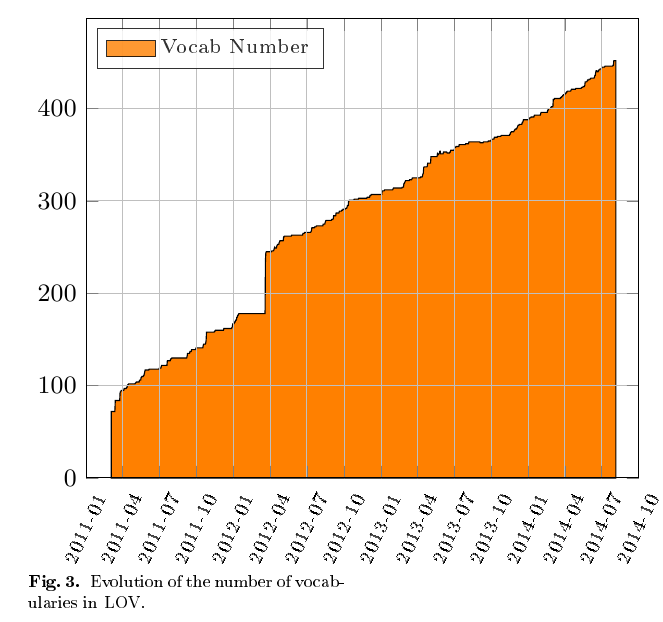
\includegraphics[width=\linewidth]{img/LOVEvol.png}
  \caption{Graph evolution of vocabularies inserted into LOV since from 2011 to 2014.}
  \label{fig:translations}
\end{figure}

LOV focuses only on vocabularies (subpart of semantic documents of the web) submitted by any user, reviewed and validated by curators. In addition, LOV keeps track of different versions of the vocabularies in the server that can be retrieved for comparing the differences between along the time evolution.  In contrast, Swoogle is designed to automatically discover Semantic Web Documents (SWDs), indexes their metadata and answers queries about it. Thus, the result of a search query retrieved any semantic document. For example, a query of the term \textit{person} gives $16,438$ results while in LOV, only the term appears in $134$ vocabularies. 
Watson works similarly to Swoogle, crawling and indexing semantic document at a small scale, explicitly distinguishing for each document (resource), concepts, properties and individuals if available. While in Swoogle  the ranking score is displayed, Watson shows the language of the resource and the size. Falcons is a keyword-based search system for concepts and objects on the Semantic Web, and is equipped with entity summarization for browsing. It is notable that Falcons limits the search only to ontologies and a recommendation feature is provided according to users' preferences. However, it does not provide any relationships between the related ontologies, nor any domain classification of the vocabularies.   
Table \ref{tab:lovfeatures} lists some key features of LOV with respect to Swoogle, Watson and Falcons.
 \begin{table}[!htb]
\centering{
\begin{tabular}{lllll}
\specialrule{1pt}{1pt}{1pt}
 \textbf{Feature}	& Swoogle & Watson & Falcons & LOV 			 \\ \specialrule{1pt}{1pt}{1pt}
Browsing ontologies	   & Yes & Yes & Yes & Yes \\ 
Scope & SWDs & SWDs & Concepts & ontologies \\
Metrics	& Ranking & Ranking & Ranking &  LOD popularity	 \\ 
Domain filtering & No & No & No & Yes \\
Comments and review 	& No & Yes & No & Only by curators	\\ 
Ranking	& Doc. based & Doc. based & Doc. based & Metric-based			\\ 
Web service access & Yes & Yes & Yes & Yes		\\ 
SPARQL endpoint	& No & No & No & Yes		\\ 
Read/Write	& Read & Read \& Write & Read &Read  	\\ 
Ontology directory & No & No & No &Yes \\
Application platform & No & No & No & Yes \\
Storage & Cache & - & - & Dump \& endpoint \\
Interaction with Contributors & No &  - & No & Yes \\

		\\ \specialrule{1pt}{1pt}{1pt}

\end{tabular}
\caption{Comparison of LOV, with respect to Swoogle, Watson and Falcons; based on part of the framework defined in \cite{AquinJoWS12}.  }
\label{tab:lovfeatures}
}
\end{table}


\subsection{LOV vs Neon Methodology}
\label{sec:Lovandneon}

 LOV is a catalog/tool that can fits well within the Neon methodology for building vocabularies and ontologies.  Based on the Neon Methodology's glossary of activities for building ontologies \cite{MC10}, LOV is relevant in four activities:
		
\begin{description}%[fragile]
		\item [Ontology Search.] Main LOV's feature is the search of vocabulary terms. These vocabularies are categorized within LOV according to the domain they address. In this way, LOV contributes to ontology search by means of (a) keyword search and (b) domain browsing.
		\item [Ontology Assessment.] LOV provides a score for each term retrieved by a keyword search. This score can be used during the assessment stage and includes a unique term statistical feature\footnote{\url{http://lov.okfn.org/dataset/lov/stats/}} which provides for each term registered in LOV the following information: (a) ``LOV distribution'' that represents the number of vocabularies in LOV that refer to a particular element; (b) ``LOV popularity'' that shows the number of other vocabulary elements that refers to a particular one; and (c) ``LOD distribution'' that refers to the number of datasets in LOD which use a particular vocabulary; and (d) ``LOD popularity'' that refers to the number of vocabulary element occurrences in the LOD.
		\item [Ontology Mapping.] As explained in section \ref{voafRelations}, vocabularies rely on each other in seven different ways. In LOV these relationships are explicitly stated using VOAF vocabulary. This data could be useful to find alignments between ontologies, for example one user might be interested in finding equivalent classes for a given class or all the equivalent classes among two ontologies. The following example shows the retrieved data when asking for all the equivalent classes and properties between the vocabularies foaf and dcterms by means of the related VOAF query\footnote{\url{http://goo.gl/sTIGQ6}. Prefixes are omitted for readability purpose. You can find the correct namespace for a prefix in LOV.}: 
				
		{\small\begin{verbatim}SELECT DISTINCT ?elem1 ?alignment ?elem2 {
				     {?elem1 <http://www.w3.org/2002/07/owl#equivalentClass> ?elem2}
				     UNION {?elem1 <http://www.w3.org/2002/07/owl#equivalentProperty> ?elem2}
				     UNION {?elem2 <http://www.w3.org/2002/07/owl#equivalentClass> ?elem1}
				     UNION {?elem2 <http://www.w3.org/2002/07/owl#equivalentProperty> ?elem1}
				     FILTER(!isBlank(?elem2))
				     FILTER(!isBlank(?elem1))
				     ?elem1 ?alignment ?elem2.
				     ?elem1 rdfs:isDefinedBy <http://xmlns.com/foaf/0.1/>.
				     ?elem2 rdfs:isDefinedBy <http://purl.org/dc/terms/>.
				} ORDER BY ?alignment\end{verbatim}}
				
	Figure \ref{fig:eqCR} shows the alignments between foaf and dcterms vocabularies by mean of \url{owl:equivalentClass} and \url{owl:equivalentProperty}. 

\begin{figure}
\centering
  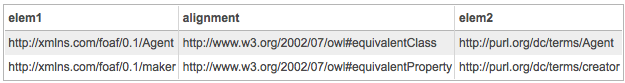
\includegraphics[width=1.0\linewidth]{img/equivalentCandR.png}
  \caption{Equivalent classes and properties between foaf and dcterms}
  \label{fig:eqCR}
\end{figure}

							
		\item [Ontology Localization.] Labels in different languages are stored in the LOV endpoint for the ontology terms that provide such information. This annotations could be used when translating terms into different languages. This information could be extracted by querying the SPARQL endpoint as in the following example\footnote{\url{http://goo.gl/JJCJ01}} where all the labels defined for the terms that have at least one \url{rdfs:label} containing strictly ``person":
		
		{\small\begin{verbatim}SELECT DISTINCT ?label2 ?element{
								     ?element rdfs:label ?label1 .
								     ?element rdfs:label ?label2 .
								     FILTER (?label1 != ?label2 ).
								     FILTER(REGEX(STR(?label1), "person", "i")).
					} ORDER BY ?element\end{verbatim}}
						 
								     
		An excerpt of the query result is shown in figure \ref{fig:translations}. From that result, ``Persona''@es and ``Personne''@fr could be used as translations for the English term ``Person'' in Spanish and French respectively.


\begin{figure}
\centering{
  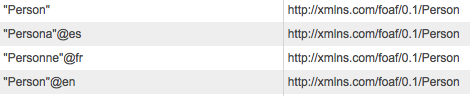
\includegraphics[width=.90\linewidth]{img/translations1.png}
  \caption{Translations example for foaf:Person}
  \label{fig:translations}
  }
\end{figure}

\end{description}

		Figure \ref{fig:LOVandNeOn} shows the activities LOV can support within the overall Neon methodologies activity workflow.
		
\begin{figure}
\centering
  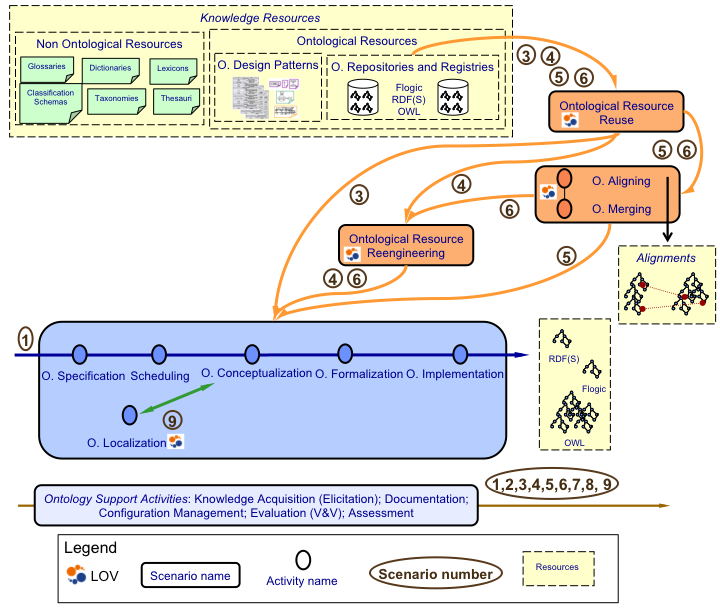
\includegraphics[width=.95\linewidth]{img/neonScenarios.png}
  \caption{Meeting points between LOV and the NeOn methodology, derived from \cite{MC10}.}
  \label{fig:LOVandNeOn}
\end{figure}


\section{Prefixes harmonization}
\label{sec:prefharmoni}

RDF vocabularies bring their meaning to linked data by defining classes and properties, and their formal semantics. Relying on W3C standards RDFS or OWL, those vocabularies are a fundamental layer in the architecture of the Semantic Web. Without the explicit semantics declared in vocabularies, linked data, even using RDF, would be just linked pieces of information where links have no meaning. Interoperability between data and datasets rely heavily on shared vocabularies, but given the distributed nature of the Web, vocabularies are published by independent parties and there is no centralized coordination of this publication, nor should it be. Various independent services have been developed in order to discover vocabularies and provide information about them, and the community of data publishers and vocabulary managers have all interest in complementarity and coordination between such services. In this section, we focus on a specific aspect of vocabularies: their identification by namespaces and associated prefixes.

In the original XML syntax of RDF, prefixes are simply local shortcuts associated with XML namespaces using \texttt{xmlns} declarations. The usage of prefixes has been further extended to other syntaxes of RDF such as N3 and Turtle. Although a prefix to namespace association is syntactically limited to the local context of the file in which it is declared, common prefixes such as \texttt{rdf:}, \texttt{rdfs:}, \texttt{owl:}, \texttt{skos:}, \texttt{foaf:} and many more have become de facto standards. For example, RDFa has 1.1 has a default profile made of 11 well-used vocabularies based on their general usage on the Semantic Web according to the crawl of Yahoo! and Sindice as of March 2013\footnote{\url{http://www.w3.org/2010/02/rdfa/profile/data/}}. Similarly, the YASGUI SPARQL editor has a list of built-in prefix-namespace associations to ease the construction of SPARQL queries. However, this list of ``standard'' prefixes is open-ended. Interfaces such as SPARQL endpoints (e.g. Virtuoso) use a list of built-in prefixes declaration for more and more namespaces but the choice of entries in this list is all but transparent. Hence, the reason of a given namespace being or not in this list could be interpreted in many ways, a potential source of technical and social conflicts. Therefore, the notion has been slowly spreading, at least implicitly, that common prefixes could and indeed should have a global use, implying some kind of governance and good practices. More and more vocabularies explicitly recommend the prefix that should be used for their namespace, generally using a common if not written good practice to avoid frontal clashes by recommending a prefix not already used. But there is no global policy except implicit rules of fair use to avoid potential conflicts resulting from polysemy (different namespaces using or recommending the same prefix) or synonymy (different prefixes used for the same namespace).

A vocabulary publisher needs to have access to some services capable of monitoring the existing prefixes usage in order to stick to those rules. Moreover, we focus on two services providing such information on prefixes usage namely prefix.cc\footnote{Service: \url{http://prefix.cc/}; Code: \url{https://github.com/cygri/prefix.cc}} and LOV (Linked Open Vocabularies)~\cite{Datalift:D22}. Both services provide associations between prefixes and namespaces but following a different logic. The prefix.cc service allows anybody to suggest a prefix to namespace association. It supports polysemy and synonymy, and has a very loose control on its crowd-sourced information. What it provides is more a measure of popularity of prefixes and namespaces than a way to put order in them. LOV has a much more strict policy forbidding polysemy and synonymy, enforced by a dedicated back-office database infrastructure, ensuring that each vocabulary in the LOV database is uniquely identified by a prefix, this unique identification allowing the usage of prefixes in various LOV publication URIs. This requirement leads sometimes to a situation where LOV uses prefixes different from the ones recommended by the vocabulary publishers.

\subsection{Aligning LOV with Prefix.cc} \label{sec:alignment}
In this section, we present how we perform the alignment between the two services LOV and prefix.cc. Figure~\ref{fig:evolution} shows the evolution of the number of prefixes registered in these two services between April 2009 and July 2013. Our main goals are to align Qnames (prefix) to a unique URI in LOV and to make sure that all the vocabularies in LOV are actually inserted in prefix.cc.

\begin{figure}[ht]
\centering
\resizebox{\textwidth}{!}{
%\documentclass{standalone}
%\usepackage{pgfplots}
%\begin{document}
\begin{tikzpicture}
\begin{axis}[
%\begin{semilogxaxis}[
 cycle list name=exotic,
 ylabel=number of prefix-namespace,
 xlabel=month,
% legend pos=outer north east,
 legend style={at={(0.02,0.98)},anchor=north west,opacity=0.6},
% legend columns=2,
 axis on top,
 ymin=0,ymax=1300,
 mark size=0pt,
 grid=major,
% minor x tick num=10,
% minor y tick num=10,
%xtick={Jan-09,Feb-09,Mar-09,Apr-09,May-09,Jun-09,Jul-09,Aug-09,Sep-09,Oct-09,Nov-09,Dec-09,Jan-10,Feb-10,Mar-10,Apr-10,May-10,Jun-10,Jul-10,Aug-10,Sep-10,Oct-10,Nov-10,Dec-10,Jan-11,Feb-11,Mar-11,Apr-11,May-11,Jun-11,Jul-11,Aug-11,Sep-11,Oct-11,Nov-11,Dec-11,Jan-12,Feb-12,Mar-12,Apr-12,May-12,Jun-12,Jul-12,Aug-12,Sep-12,Oct-12,Nov-12,Dec-12,Jan-13,Feb-13,Mar-13,Apr-13,May-13,Jun-13,Jul-13,Aug-13},
xtick={Jan-09,Apr-09,Jul-09,Oct-09,Jan-10,Apr-10,Jul-10,Oct-10,Jan-11,Apr-11,Jul-11,Oct-11,Jan-12,Apr-12,Jul-12,Oct-12,Jan-13,Apr-13,Jul-13},
 ytick={0,100,...,1300},
 symbolic x coords={Jan-09,Feb-09,Mar-09,Apr-09,May-09,Jun-09,Jul-09,Aug-09,Sep-09,Oct-09,Nov-09,Dec-09,Jan-10,Feb-10,Mar-10,Apr-10,May-10,Jun-10,Jul-10,Aug-10,Sep-10,Oct-10,Nov-10,Dec-10,Jan-11,Feb-11,Mar-11,Apr-11,May-11,Jun-11,Jul-11,Aug-11,Sep-11,Oct-11,Nov-11,Dec-11,Jan-12,Feb-12,Mar-12,Apr-12,May-12,Jun-12,Jul-12,Aug-12,Sep-12,Oct-12,Nov-12,Dec-12,Jan-13,Feb-13,Mar-13,Apr-13,May-13,Jun-13,Jul-13,Aug-13},
 xmin=Feb-09,xmax=Aug-13,
 x tick label style={rotate=65,anchor=east,font=\scriptsize}
 ]
  
\pgfplotstableread{PGFPlots/prefixcc-lov-evo.dat}\thisTable
%\pgfplotstableread{prefixcc-lov-evo.dat}\thisTable

\addplot table[x=month,y=prefix.cc]{\thisTable};
\addlegendentry{prefix.cc}

\addplot table[x=month,y=LOV]{\thisTable};
\addlegendentry{LOV}

%\end{semilogxaxis}
\end{axis}
\end{tikzpicture}
%\end{document}
}
\vspace{0.1cm}
\caption{Evolution of the number of prefix-namespace pairs registered in prefix.cc and LOV}
\label{fig:evolution}
\end{figure}

We propose to perform SPARQL queries over all the files of prefix.cc at\\
 \url{http://prefix.cc/popular/all.file.vann} in the FROM clause and compare them to the content of the LOV SPARQL endpoint\footnote{\url{http://lov.okfn.org/endpoint/lov}} via a SERVICE\footnote{\url{http://www.w3.org/2009/sparql/docs/fed/service}} call. The SERVICE keyword defined in the SPARQL 1.1 Query Language instructs a federated query processor to invoke a portion of a SPARQL query against a remote SPARQL endpoint~\cite{eric2013}. Results are returned to the federated query processor and are combined with results from the rest of the query. To be more generic and standards-compliant, the queries could be run with the Jena ARQ command-line tool to produce a CSV or a JSON serialization that could be easily consumed either by the prefix.cc backend via phpMyAdmin or by the LOV backend.

\subsection{First Task: prefixes in LOV not present in Prefix.cc}  \label{sec:notInPrefix}
First, we compute $<LOV> INTERSECTS <PREFIX.CC>$ and $<LOV> MINUS \, \{<LOV> INTERSECTS <PREFIX.CC> \}$. The following SPARQL query finds namespace URIs in LOV that do not exist in prefix.cc along with their LOV prefix.
\begin{verbatim}
PREFIX vann: <http://purl.org/vocab/vann/>
SELECT ?prefix ?lovURI
FROM <http://prefix.cc/popular/all.file.vann> {
  SERVICE <http://lov.okfn.org/endpoint/lov> {
    SELECT ?prefix ?lovURI {
      [] vann:preferredNamespacePrefix ?prefix;
        vann:preferredNamespaceUri ?lovURI;
    }
  }
  FILTER (NOT EXISTS { [] vann:preferredNamespaceUri ?lovURI })
  OPTIONAL {
    [] vann:preferredNamespacePrefix ?prefix;
      vann:preferredNamespaceUri ?pccURI;
  }
}
ORDER BY ?prefix
\end{verbatim}
The first results\footnote{This query was performed in two weeks between March, 2nd and March, 20th 2013 and at this time, card(LOV) = 321 vocabularies while card(Prefix.cc) = 925} shown the following: $card(LOV) \bigcap card(PREFIX.cc) = 188$\footnote{\url{http://www.eurecom.fr/~atemezin/iswc2013/experiments/firstAlignments/intersection-prefixLOV-02-03.csv}} and $card (LOV) - card( PREFIX.cc) = 133$\footnote{\url{http://www.eurecom.fr/~atemezin/iswc2013/experiments/firstAlignments/inLovNotINPrefixcc-02-03.csv}} prefixes in LOV not yet registered in prefix.cc. At this point, a first batch of $80$ prefixes/namespaces from LOV were safely imported in prefix.cc since there were no conflicts. For the remaining conflicting ones, they needed more in-depth analysis.

\subsection{Second Task: Dealing with Conflicts between Prefix.cc and LOV}  \label{sec:conflicts}
In the process of alignment, there were two types of conflicts and we provide appropriate actions and/or solutions accordingly:
\begin{itemize}
 \item Clashes: cases where we have in both services the same prefix but different URIs;
 \item Disagreements on preferred namespace: cases where for the same URI, we found different prefixes.
\end{itemize}

\subsubsection*{Clashes.} We performed a SPARQL query as above to identify clashes in vocabularies ($30$). In Table~\ref{tab:clashes-types}, we identify seven different types of issues to deal with, such as (i) real conflicts, (ii) URIs are 404, (iii) URIs are obsolete versions and (iv) two URIs redirecting to the same resource.
\begin{table}
\centering{
\begin{tabular*}{14cm}{lcl}
\specialrule{1pt}{1pt}{1pt}
 \textbf{Type of issue}	& \textbf{\# Vocabularies} 	& \textbf{\%} 		 \\
 \specialrule{1pt}{1pt}{1pt}
 pccURI and lovURI redirect to same resource  & 8 	& 26.67\%		\\
 lovURI already in prefix.cc as secondary	  & 7   & 23.3\%  		\\
 Real conflicts 	                & 6 			& 20\% 	 		\\
 pccURI is 404	                    & 4 			& 13.3\%		\\
 pccURI is an obsolete version		& 3   			& 10\%  		\\
 lovURI is 404		                & 1   			& 3.3\%  		\\
 lovURI is an obsolete version		& 1   			& 3.3\%  		\\
 \specialrule{1pt}{1pt}{1pt}
\end{tabular*}
\caption{Type of issues encountered for vocabulary clashes}
\label{tab:clashes-types}
}
\end{table}

\subsubsection*{Disagreements on namespace URIs.} The general idea is that if vocabulary editors have not included explicitly a \\ \texttt{vann:preferredNamespacePrefix} in their description, the curators of LOV are free to change it and put whatever seems appropriate. At the same time, in prefix.cc, having multiple prefixes for the same namespace IRI in not a problem. However, we computed those prefixes in LOV that have different prefixes in prefix.cc. The following query retrieves the URIs falling in those disagreements:
\begin{verbatim}
PREFIX vann: <http://purl.org/vocab/vann/>
SELECT ?prefix ?lovURI ?prefixcc
FROM <http://prefix.cc/popular/all.file.vann> {
  SERVICE <http://lov.okfn.org/endpoint/lov> {
    SELECT ?prefix ?lovURI {
      [] vann:preferredNamespacePrefix ?prefix;
        vann:preferredNamespaceUri ?lovURI;
    }
  }
  FILTER (?pccURI = ?lovURI && ?prefix != ?prefixcc)
  OPTIONAL {
    [] vann:preferredNamespacePrefix ?prefixcc;
      vann:preferredNamespaceUri ?pccURI;
  }
}
ORDER BY ?prefix
\end{verbatim}
From the results of this query ($61$ cases), we have three actions to perform:
\begin{itemize}
  \item add the lovPrefix (prefix in LOV) in prefix.cc (e.g: adding \\\texttt{geod}:\texttt{http://vocab.lenka.no/geo-deling\#}) to the existing \texttt{ngeoi} in \textit{pccPrefix}.)
  \item add more alternative URIs to the existing prefix in prefix.cc (e.g: adding \texttt{prov}:\texttt{http://purl.org/net/provenance/ns\#}) to the existing \texttt{hartigprov, prv} in \textit{pccPrefix})
  \item change a prefix in LOV\footnote{\url{http://www.eurecom.fr/~atemezin/iswc2013/material/action-sameUriDifferentPrefixes.pdf}} (e.g: lovPrefix \texttt{dc} for \texttt{http://purl.org/dc/terms} not in the list $\{dcterm, dcq, dct, dcterms\}$ has been replaced by \texttt{dce} in LOV).
  \item No changes when the lovPrefix is contained in the set of prefixes of prefix.cc.
\end{itemize}

\subsection{Social Aspects} \label{sec: social}
Several vocabularies are maintained by a community of users. As part of the alignment process, we contacted the authors, creators or maintainers (if they exist) of vocabularies to involve them as well in the process of changing prefixes, and agree with them to fix some issues regarding their vocabularies. From the homepages of the vocabulary authors and editors collected in LOV, we connect to their social platform accounts such as LinkedIn, Google+ or Twitter. Table~\ref{tab:contact-editors} summarizes some cases of real conflicts where the LOV curators have to find and contact the editors of the vocabularies for negotiation.

\begin{table}[htp]
\centering{
\begin{tabular*}{12cm}{lll}
 \specialrule{1pt}{1pt}{1pt}
 prefix & lovURI		& Remark \\
 \specialrule{1pt}{1pt}{1pt}
 sp & \scriptsize{http://data.lirmm.fr/ontologies/sp\#} &	 contact editor at LIRMM ($sp \Rightarrow osp$) \\  %\scriptsize{http://spinrdf.org/sp\#}
 scot & \scriptsize{http://scot-project.net/scot/ns\#} &  contact editors at lovURI \\   % \scriptsize{http://scot-project.org/scot/ns\#} &
 media &	\scriptsize{http://purl.org/media\#}	 & contact editors for negotiation \\ %& \scriptsize{http://purl.org/microformat/hmedia/}
 pro	& \scriptsize{http://purl.org/spar/pro/}  &  contact editors for negotiation \\   % &	\scriptsize{http://purl.org/hpi/patchr\#}
 swp	& \scriptsize{http://www.w3.org/2004/03/trix/swp-1/}  & contact editors, fix on LOV side \\  %& \scriptsize{http://www.w3.org/2004/03/trix/swp-2/}
 wo & \scriptsize{http://purl.org/ontology/wo/core\#}	 & contact editors \\  %& \scriptsize{http://purl.org/ontology/wo/}
 idemo &	\scriptsize{http://rdf.insee.fr/def/demo\#}	 & to resolve with INSEE \\ %& \scriptsize{http://rdf.insee.fr/graphes/def/demo\#}
 \specialrule{1pt}{1pt}{1pt}
\end{tabular*}
\caption{LOV and prefix.cc conflicts resolution leading to contact vocabularies editors for negotiation. We provide the prefix, the URI in LOV and the action undertaken.}
\label{tab:contact-editors}
}
\end{table}

%%%%%%%%%%%%%%%%%%%%%%%%%%%%%%%%%%%%%%%%%%%%%%
%%%  4. Finding Vocabularies in Prefix.cc  %%%
%%%%%%%%%%%%%%%%%%%%%%%%%%%%%%%%%%%%%%%%%%%%%%

\subsection{Finding Vocabularies in Prefix.cc}   \label{sec:finding}
We want to find out in prefix.cc, which of the couples (prefix, URI) could be potentially a vocabulary to be further assess to be included in the LOV catalog. To address this question, we first compute all the differences on prefix.cc NOT in LOV, i.e. $PREFIX.CC$ MINUS $(LOV <INTERSECT> PREFIX.CC)$, performing using a SPARQL query. This results in $742$ URIs to be checked\footnote{\url{http://www.eurecom.fr/~atemezin/iswc2013/experiments/input/notInLOV.json}}.

\subsubsection{LOV Check API}
We have implemented an API\footnote{\url{http://lov.okfn.org/dataset/lov/apidoc/}} that allows a user to run the LOV-Bot over a distant vocabulary. It takes as parameter the vocabulary URI to process and the time out (integer) specified to stop the process. The result of this action is a set of $26$ property-values from which we are interested in using only $8$ of them, namely:
\begin{itemize}
 \item \textbf{uri} (string); uri of the vocabulary.
 \item \textbf{namespace} (string) ; namespace of the vocabulary.
 \item {\textbf{prefix} (string) ;  prefix of the vocabulary}
 \item{\textbf{inLOV} (boolean) ; indicates if the vocabulary is already in the Linked Open Vocabularies ecosystem}.
 \item {\textbf{nbClasses} (int) ; Number of classes defined in the vocabulary namespace}.
 \item{\textbf{nbProperties} (int) ; Number of properties defined in the vocabulary namespace}.
 \item{\textbf{dateIssued }(string) ; Vocabulary date of issue}.
 \item{\textbf{title} (Taxonomy) ; List of titles with language information if available}.
\end{itemize}

The code below gives the response of our algorithm for the vocabulary identified at \url{http://ns.aksw.org/Evolution/}.
\begin{verbatim}[caption={Sample output of a response of the Check API}]
{
 "dateIssued": "None",
 "inLOV": false,
 "namespace": "http://www.agfa.com/w3c/2009/clinicalProcedure#",
 "nbClasses": 47,
 "nbProperties": 29,
 "pccURI": "http://www.agfa.com/w3c/2009/clinicalProcedure",
 "prefix": "clinproc",
 "title": [
   {
     "dataType": null,
     "language": "en",
     "value": "Clinical Procedure"
   }
 ],
 "uri": "http://www.agfa.com/w3c/2009/clinicalProcedure"
},
\end{verbatim}

\subsubsection{Experiments} \label{experiments}
We wrote a script calling the LOV Check API on the URIs in prefix.cc for determining the candidates vocabularies to be inserted in LOV using the algorithm in Listing~\ref{findvocabInPrefix-algorithm}. We ran four times the experiments (possibly due to some network instabilities) in order to determine from which results what should be assessed. Table~\ref{tab:experiment-choice} gives an overview of the number of URIs with respectively the attribute ``inLOV=false''(TP), ``inLOV=true''(FP) and the errors occurred (Null returned, http/proxy or time out reached by the API).

Regarding the experiments, \texttt{Experiment4} gives stable results with less network errors. Therefore, we stick on this experiment to report our findings and analysis. We found that $227$ ($43.48$\%) are vocabularies in the sense of LOV since they have at least one property or one class. $297$ vocabularies ($56.51$\%) might have some problems (or are even not vocabularies at all) as they have neither classes nor properties. Regarding the presence of prefixes, we found $140$ ($61.67$\%) of them.
\begin{table}[!htbp]
\centering{
\begin{tabular}{lccc}
 \specialrule{1pt}{1pt}{1pt}
 				& TP(inLOV=false) 	& FP(inLOV=true) 	& Errors	 \\
 \specialrule{1pt}{1pt}{1pt}
 Experiment1 	& 525 				& 44 				& 173 		 \\
 Experiment2 	& 403 				& 26				& 313 		 \\
 Experiment3 	& 351 				& 28				& 363 		 \\
 Experiment4	& $522$   			& 44   				& 176 		 \\
 \specialrule{1pt}{1pt}{1pt}
\end{tabular}
\caption{Experiments looking for stable results of finding vocabularies in prefix.cc.}
\label{tab:experiment-choice}
}
\end{table}
The $227$ vocabularies could all be inserted in the LOV catalog since they fulfill the current requirements of what is a `` LOV-able vocabulary''. In this list, we found vocabularies such as \texttt{rdf, rdfs, owl} that are used to build other vocabularies but are not yet integrated in the LOV catalog.

\begin{algorithm}[H]
\caption{finding vocabularies NOT in LOV from prefix.cc algorithm} 
\label{findvocabInPrefix-algorithm}
\begin{algorithmic}[1]
    \STATE Open $notInLOV.json$ file containing the prefix.cc URIs \emph{NOT} in LOV 
    \STATE initialize $item$ as List
    \STATE Initialize $result$ as collection of $item$
    \FOR { each $pccURI \in notInLOV file$}
      \STATE $uri \leftarrow$ value of $pccURI$
      \STATE $uriv \leftarrow$ construct-valid $uri$
      \STATE call LOV-Check API with parameter $uriv$
      \STATE try/catch HTTPError, URLError, IOError, ValueError
      \WHILE { no error raised}
        \STATE initialize $item$ to an empty List
        \STATE append $pccURI, prefix, inLOV, namespace, title, dateIssued, nbClasses, nbProperties$ in $item$ List
        \STATE append $item$ to $result$
      \ENDWHILE
    \ENDFOR
    \STATE RETURN $output-result$
\end{algorithmic}
\end{algorithm}

From the list of URIs that were not LOV-able vocabularies, we wanted to do more analysis by checking the RDF files using the Triple-Checker tool. Our aim is to be sure if we did not leave out some candidate vocabularies or if there are other type of errors such as parsing errors. Table~\ref{tab:triplechecker-analysis} provides results classified into $4$ categories:
\begin{itemize}
 \item General errors such as loading files or proxy errors: 78.30\%
 \item Candidate LOV-able vocabularies: 12.20\%
 \item Clearly not vocabularies ($\texttt{nbClasses} = \texttt{nbProperties} = 0 $), typically instances, datasets, html pages: 6.45\%
 \item Others (mainly parsing errors): 3.05\%
\end{itemize}

\begin{table}
\centering{
\begin{tabular}{lccc}
 \specialrule{1pt}{1pt}{1pt}
 \textbf{Total URIs }				& $295$ & 100\% 		\\
 \specialrule{1pt}{1pt}{1pt}
 Loading/404 errors			        & $182$ & 61.69\%		\\
 Vocabularies 						& 36 	& 12.20\% 		\\
 Proxy errors				        & 27   	& 9.15\%   		\\
 50x, 40x errors				    & 22   	& 7.45\%   		\\
 Parsing errors				        & 9   	& 3.05\%   		\\
 Web Pages containers				& 9   	& 3.05\%   		\\
 No triples found				    & 8   	& 2.71\%   		\\
 RDF data 						    & 2 	& 0.67\%		\\
\specialrule{1pt}{1pt}{1pt}
\end{tabular}
\caption{Analysis of the URIs with no classes and no properties while using the LOV-Bot API}
\label{tab:triplechecker-analysis}
}
\end{table}

\subsection{Conclusion}    \label{sec:conclusion}
In this Section, we have analyzed numerous vocabularies referenced in LOV and in prefix.cc and we have presented a way to manage the prefixes of those vocabularies. We have shown that in the process of mapping namespaces with prefixes, some conflicts have to be resolved, often by contacting the editors themselves. One future work is to develop a new strategy for the LOV-Bot API to take into account vocabularies published in other formats such as n3 and turtle. This would require to first test the validity of those formats and to adapt the way namespaces are obtained in order to not check only the presence of the \texttt{vann:preferredNamespace} property but to rely on similarity algorithm in order to guess the closest namespace given a URI vocabulary and some statistics of the number of classes and properties.

The work can be extended in several directions. Sticking to the two services we have studied and already contributed to harmonize, the possible next steps would be to automate as far as possible the tasks that have been made semi-automatically so far: \emph{i)} developing a unique interface for submitting namespaces and prefixes to both services; \emph{ii)} bridging the LOV back-office and the prefix-cc database using both services API in order to publish a list of common recommended prefixes. The latter goes beyond the limited framework of the two original services since such a list could be consolidated and endorsed by the main actors in vocabulary publication and management, and recommended for use in linked data applications. This could be picked up by the upcoming W3C Vocabulary Management Working Group as part of the new Data Activity\footnote{\url{http://www.w3.org/2013/05/odbp-charter.html}}.
 
This (apparently) simple issue of prefixes and namespaces is providing a good illustration of why some kind of governance is needed in the distributed ecosystem of vocabularies and linked data, pointing to both technical and social aspects, and proposing concrete examples of conflict resolution. There is no, and certainly there should never be any, central attribution authority for prefixes, and the needed regulation has to be made a posteriori, including good practices of cooperation and negotiation between vocabulary publishers. Development and harmonization of services such as LOV and prefix.cc is then to be considered as part of the current and more general effort already started by the DCMI\footnote{Long-term Preservation and Governance of RDF Vocabularies: \url{http://dcevents.dublincore.org/IntConf/index/pages/view/vocPres}} and W3C\footnote{W3C Vocabulary Services: \url{http://www.w3.org/2013/04/vocabs/}} for a sustainable governance of vocabularies.

\section{Vocabulary Ranking metrics}
\label{sec:vocabranking}

\label{sec:introduction}
The linked data principles have gained significant momentum over the last few years as a best practice for sharing and publishing structured data on the Semantic Web~\cite{Bizer2009}. Before being published, data is modeled and ontologies or vocabularies are one of the key elements of a dataset. Vocabularies are the artefact that bring semantics to raw data. One of the major barriers to the deployment of linked data is the difficulty for data publishers to determine which vocabularies should be used since developing new vocabularies has a cost. Catalogues of ontologies are therefore a useful resource for searching terms (classes and properties) defined in those vocabularies. The Linked Open Vocabulary (LOV) initiative~\cite{scharffe_2012} is playing a significant role in providing such services to users who can search within curated vocabularies, fostering ontologies reuse. LOV focuses only on vocabularies submitted by users, which are then reviewed and validated by curators. In addition, LOV computes dependencies between vocabularies, keeps track of different versions of them in order to enable their temporal evolution.

To the best of our knowledge, recommending vocabularies to reuse are limited to ``popular'' or ``well-known'' ones. This paper proposes a metric combining different features such as how vocabularies are interlinked, or how they are used in real world datasets. This contribution originates also in the desire to bring the traditional concept of Information Content (IC) into the field of the semantic web applied to vocabularies. Many catalogs of ontologies already provide some ranking metrics based on some features. However, we are interested in applying the principles of IC on vocabularies to investigate if such techniques can give more insights in ontology ranking and ontology usage (e.g in visualization applications).

This Section is organized as follows: Section~\ref{sec:theory} defines the theory of Information Content, and the features used for applying Partition Information Content to vocabularies. We present our experiments on the LOV catalogue in the Section~\ref{sec:experiments}. We discuss how this ranking metric can be used for vocabulary design and maintenance in Section~\ref{sec:application}. We compare our results with other rankings for vocabularies in Section~\ref{sec:related} before concluding and outlining future work (Section~\ref{sec:conclusion}).



\subsection{Information Content Metrics}
\label{sec:theory}
Based on probability theory, Information Content (IC) is computed as a measure of generated amount of surprise~\cite{ross02}. More common terms in a given corpus with higher chance of occurrence cause less surprise and accordingly carry less information, whereas infrequent ones are more informative. We reuse the notion of informativeness as the value of information associated with a given entity, where Information Content has a negative relation with its probability. The concept of Information Content can be used to rank each entity, term, or alphabet in the corpus. We apply the Partitioned Information Content to measure the informativeness of Linked Open Vocabularies as a semantic network of resources connected together using different range of relations, as described in~\cite{Meymandpour13}. Partitioned Information Content (PIC) is derived from the IC value using some weights. We empirically set those weights according to three features:
\begin{itemize}
 \item (i) datasets using the vocabulary ($weight = 2$);
 \item (ii) \textit{outlinks} from a vocabulary, i.e. whether a vocabulary reused other vocabularies ($weight = 1$);
 \item (iii) \textit{inlinks} to a vocabulary, i.e. whether other vocabularies are reusing this vocabulary ($weight = 3$).
\end{itemize}

\subsection{Information Content in Linked Open Vocabularies}
This experiment aims at bringing the concept of informativeness in the field of terms semantically related as it is the case within semantic web ontologies. The ranking obtained can give additional information based on the Information Content theory to help reusing terms and detecting the ones that are less popular. This can then be used by applications consuming datasets described with these vocabularies. The equation (1) gives the formula for computing the IC value of a term (class or property):
\begin{equation}
 IC(t) = -\log_2(\frac{\varphi(t)}{N}) ,
\end{equation}
where $N$ is set to be the maximum value corresponding to the term occurrence in the LOV aggregator (as of June 2014, this value is $3958$, and it corresponds to the popularity of the \texttt{skos:prefLabel} property); and $\varphi(t)$ is the occurrence of the term (but not its popularity).

For computing $\varphi(t)$, we use two types of SPARQL queries depending on whether the term is a class (Listing~\ref{list:classCount}) or a property (Listing~\ref{list:propCount} considers \texttt{owl:ObjectProperty}, \texttt{owl:Data\-typeProperty} and \texttt{rdfs:Property}). Note that we do not yet take into account the \texttt{owl:equivalentClass} and \texttt{owl:equi\-valentProperty} axioms that may appear in some vocabularies. We leave this as a future work.

\begin{lstlisting}[float=htb,caption={SPARQL query for computing the occurrence of a class },label=list:classCount]
 SELECT (count(?uri1) as ?occ)
 WHERE {
   ?uri1  ?p %%classURI . }
\end{lstlisting}

\begin{lstlisting}[float=htb,caption={SPARQL query for computing the occurrence of a property },label=list:propCount]
 SELECT (count(?uri1) as ?occ)
 WHERE {
   ?uri1 +objectURI+ ?uri2.
   FILTER  (?uri1 != ?uri2) }
\end{lstlisting}

\subsection{Ranking Vocabularies using Information Content}
For computing the PIC value, we use the following formula:
\begin{equation}
 PIC(f) =  w_{f} \times \sum_{i=1}^{n}IC(t_{i})  ,
\end{equation}
where $w_{f}$ is the weight related to vocabulary $f$.

We consider very important that a vocabulary is being reused by other vocabularies and implemented within real world datasets. For example, the \texttt{foaf} ontology is weighted $6$ because it reuses vocabularies (1), it has been used in some datasets (2) and it is being reused by other vocabularies (3). The \texttt{dul}\footnote{\url{http://www.ontologydesignpatterns.org/ont/dul/DUL.owl}} vocabulary is weighted $3$ because it doesn't reuse any vocabulary but it is instead used by several other vocabularies.
\vspace{-0.2cm}

%%%%%%%%%%%%%%%%%%%%%%%%%%%%%%%%%%%%%%%%
%%%   Experiments on Vocabularies  %%%
%%%%%%%%%%%%%%%%%%%%%%%%%%%%%%%%%%%%%%%%

\subsection{Experiments on Vocabularies}
\label{sec:experiments}
We use the LOV catalogue, and particularly the LOV aggregator\footnote{\url{http://lov.okfn.org/endpoint/lov_aggregator}} to look at the terms (classes and properties) to compute their Information Content (IC). LOV defines the \textit{LOV Distribution} as the number of vocabularies in LOV that refer to a particular element and the \textit{LOV popularity} as the number of other vocabulary elements that refers to a particular one. Based on the concept of Partitioned Information Content, we implement our ranking measure according to the algorithm~\ref{rankingvocab}. We take the subset of classes and/or properties with LOV popularity and LOV distribution greater than one. The initial set of vocabularies in LOV is $366$. After filtering the candidate terms, we came out with a set of $161$ vocabularies ($44\%$ or $161$ vocabularies) for computing their ranking.

The Table~\ref{tab:top15} gives the Top 15-ranking of the vocabularies according to the informativeness of the classes and properties used within the LOV ecosystem. As the function is proportional to the number of terms, we use a threshold of $22$ terms in the vocabularies. For example, the PIC value of \texttt{dcterms} is higher than \texttt{foaf}'s because the former uses $53$ terms (39 properties and 14 classes), while the latter only $35$ terms (9 classes and 26 properties), although they both have the same weight value.

The Table~\ref{tab:top20} shows the Top 20 namespaces of vocabularies according to the informativeness of the classes and properties used within the LOV ecosystem, along with their Information Content Value.
\begin{table}[htbp]
\centering{
\begin{tabular}{lrcc}
\specialrule{1pt}{1pt}{1pt}
 \textbf{Rank}	& \textbf{Prefix} 	& \textbf{PIC score} 		 \\ \specialrule{1pt}{1pt}{1pt}
1 	& \textsf{dcterms}			& 1724.844	 		 \\
2	& \textsf{schema}		    & 1588.700				 \\
3 	& \textsf{gr} 				& 1261.101		\\
4	& \textsf{foaf}  			& 1033.197 			\\
5	& \textsf{bibo}   			& 876.205  			\\
6	& \textsf{time}   			& 816.2020  			\\
7	& \textsf{skos}   			& 805.287  			\\
8	& \textsf{dul}   			& 797.328  			\\
9	& \textsf{ptop}   			& 773.167  			\\
10	& \textsf{rdafrbr}   		& 640.834 			\\
11	& \textsf{vaem}   		    & 630.621 			\\
12	& \textsf{ma-ont}   		& 508,694 			\\
13	& \textsf{prov}   		    & 497.524 			\\
14	& \textsf{swrc}   		    & 437.394 			\\
15	& \textsf{dce}   			& 428.618  			\\ \specialrule{1pt}{1pt}{1pt}
\end{tabular}
\caption{Top 15 vocabularies according to their PIC. All the prefixes used for the vocabularies are the ones used by LOV}
\label{tab:top15}
}
\end{table}

\begin{table}[htbp]
\centering{
\begin{tabular}{llr}
\specialrule{1pt}{1pt}{1pt}
 \textbf{Rank}	& \textbf{vocab term} & \textbf{IC value} 			 \\ \specialrule{1pt}{1pt}{1pt}
1 	& \textsf{skos:example}	& 7.7806		       	 		 \\
2	& \textsf{dce:contributor} & 4.674						 \\
3 	& \textsf{skos:scopeNote} & 4.365					\\
4	& \textsf{dcterms:source} & 4.299			 			\\
5	& \textsf{mads:code}   	& 3.922		  			\\
6	& \textsf{mads:authoritativeLabel}  & 3.922 			\\
7	& \textsf{vs:userdocs} 	& 3.847		 			\\
8	& \textsf{dce:title}  & 3.79			  			\\
9	& \textsf{skos:hasTopConcept} & 3.4547 		 		\\
10	& \textsf{dce:description} & 2.758 		 		\\
11	& \textsf{dcterms:issued} & 2.553	 		\\
12	& \textsf{dce:creator}	& 2.518 		\\
13	& \textsf{skos:inScheme}	& 2.202 		\\
14	& \textsf{skos:notation}	& 1.924	 		\\
15	& \textsf{dcterms:description} & 1.646		 		\\
16	& \textsf{coll:List}		& 0.761		\\
17	& \textsf{vs:term\_status}	& 0.735	 		\\
18	& \textsf{skos:definition}	& 0.43	 		\\
19	& \textsf{skos:prefLabel} & 0.009	 		\\
20	& \textsf{foaf:Person} & 0		  			\\ \specialrule{1pt}{1pt}{1pt}
\end{tabular}
\caption{Ranking of Top 20 terms (classes and properties) according to their IC value}
\label{tab:top20}
}
\end{table}

\begin{algorithm}[h]
\caption{Ranking vocabularies algorithm} \label{rankingvocab}
\begin{algorithmic}[1]
   \STATE REQUIRE Dump of $lov aggregator$ file
    \STATE Upload in a triple store for querying
    \STATE Select subset of candidate vocabs $ LOV aggregator endpoint $
    \FOR { $term \in lovaggregator$ }
    	\IF {($LOV distribution \geq 1$ )\AND ($LOV Popularity \geq 1$)}
     		\STATE $candidateterms \leftarrow$ append $term$
       \ENDIF
    \ENDFOR
    \FOR { each $term \in candidateterms$}
	\STATE GROUP BY vocabulary namespace
	\STATE COMPUTE weight for each vocabulary
    \ENDFOR
    \STATE INITIALIZE $PICvector$ AS a vector
     \FOR { each $term \in candidateterms$}
      \WHILE { $term \in vocabularySpace $}
        \STATE $ICterm \leftarrow$ function IC(term, vocabPrefix)
	\STATE $ICvocab \leftarrow$ $\sum ICterm $
       \ENDWHILE
        \STATE  $PICvocab \leftarrow$ $weight(vocab) \times $ICvocab
        \STATE $PICvector \leftarrow$ append (PICvocab)
        \STATE ORDER PICvector
    \ENDFOR
    \STATE RETURN PICvector
  
\end{algorithmic}
\end{algorithm}



\subsection{Application of Information Content on Vocabularies}
\label{sec:application}
We foresee various applications using the ranking method based on the Information Content metric while designing semantic web applications, vocabulary life-cycle management or novel recommendation services. We make the following recommendations when using the PIC ranking method on vocabularies:
\begin{itemize}
 \item Vocabularies on the Top PIC-ranking can be used in visualization applications, i.e. to be displayed to the user as much as possible.
 \item Terms with lower IC can be used in facetted browsing, and they seem appropriate for generating \texttt{sameAs} links during the interconnection and enrichment process. They might also be used for promoting the reuse of terms in vocabularies in general.
 \item The PIC-ranking could help the ontology designers to monitor and to assess the usage of some terms and lead to update the ontology accordingly. For example, it can be useful in extending the use of the properties such as \texttt{vs:term\_status} or \texttt{owl:deprecated}.
 \item Such a ranking can be used to rank organizations or publishers of vocabularies in a time period (e.g. annual) as a way to encourage good qualities vocabularies and/or datasets on the cloud.
\end{itemize}
The use of the information content on LOV vocabularies can be applied in the datasets interlinking task and visualization applications workflow. For interlinking datasets, this method can help detecting properties with a lower PIC which will be a candidate for the interlinking tool. The PIC score can further be used to track the vocabularies terms status (i.e. \texttt{vs:term\_status} ) or \texttt{owl:deprecated} properties by dataset maintainers. From the list of namespaces having deprecated terms (Table~\ref{tab:deprecated}), we observe some correlations with the PIC rank for the vocabularies \texttt{dcat (8), vcard (36), gr (6), wl (2), pav (1)} and \texttt{bibo (1)}\footnote{As of June 2014, there are 60 terms deprecated in LOV with the query \url{http://bit.ly/1aqcDf3}}. More precisely, the presence of \texttt{gr} and \texttt{bibo} provides evidence of such a correlation, while the presence of \texttt{dcat} and \texttt{card} can be explained by the fact that those two vocabularies are in a review process at W3C and subject to re-modeling respectively. Table~\ref{tab:deprecated} gives an overview of some namespaces with their deprecated terms.



\subsection{Related Work and Discussion}
\label{sec:related}
In this section, we look at three other catalogues providing rankings for vocabularies: vocab.cc, LODStats and prefix.cc. vocab.cc\footnote{\url{http://vocab.cc/v/tco}} does not provide a ranking for vocabularies but rather proposes a rank for classes and properties. The proposed ranking presented in Table~\ref{tab:compareRanking} is taken from the ranking of classes assuming the namespace is used only once per class.

\begin{table}[!htbp]
\centering{
\begin{tabular}{lcc}
\specialrule{1pt}{1pt}{1pt}
 \textbf{prefix}	& \#DeprecatedTerms 	& dcterms:modified		 \\ \specialrule{1pt}{1pt}{1pt}
\textsf{vcard} 	& 36	 & 2013-09-25  \\
\textsf{dcat} 	& 8 & 	2013-09-20  \\
\textsf{gr}	 & 6 & 	2011-10-01  \\ 		
\textsf{wl}	 & 2 & 	2013-05-30  \\ 	
\textsf{pav}	 & 1 & 	2013-08-30  \\ 	
\textsf{bibo	} & 1 & 	2009-11-04 	\\ \specialrule{1pt}{1pt}{1pt}
\end{tabular}
\caption{Sample of vocabularies with terms deprecated in LOV}
\label{tab:deprecated}
}
\end{table}

\begin{table}[htbp]
\centering{
\begin{tabular}{lcccc}
\specialrule{1pt}{1pt}{1pt}
 \textbf{Rank}	& \textbf{LOV-PIC } 	& \textbf{prefix.cc} 	& \textbf{vocab.cc} & \textbf{lodstats}	  \\ \specialrule{1pt}{1pt}{1pt}
1 	& dcterms			 & yago	 	& intervals	  & 	rdf		\\
2	& schema 		 & rdf		& foaf	 & rdfs			\\
3 	& gr 				& foaf		& time      	& owl			\\
4	& foaf  			& dbp 		& qb  	& dcterms			\\
5	& bibo   			& dce  		& scovo	& skos			\\
6	& time   			& owl 		& freebase  & foaf		\\
7	& skos   			& rdfs  		& mo 	 & dce		\\
8	& dul   			& dbo  		& owl	 & void			\\
9	& ptop   			& rss 		& metalex	 & geo			\\
10	& rdafrbr   		& skos 		& doap	 & aktors		\\
11	& vaem   		        & gldp 		& prov	& ro			\\
12	& ma-ont   		& geo 		& void	& obo			\\
13	& prov   		        & sc 			& frbr     	& app			\\
14	& swrc   		        & fb 			& skos       & repo 			\\
15	& dce   			& gn  		& dcterms  & time 	\\ \specialrule{1pt}{1pt}{1pt}
\end{tabular}
\caption{Comparing ranking position when using PIC in LOV with respect to prefix.cc and vocab.cc}
\label{tab:compareRanking}
}
\end{table}

The LODStats ranking is focused on covering the number of datasets reused in the linked open data cloud~\cite{demter:2012}, which is partially taken into account in our approach. The evidence of that is the first three vocabularies used (\texttt{RDF, RDFS, OWL}) which are considered as the meta model for designing vocabularies. Those vocabularies are not included into the LOV catalog and they do not appear in our ranking. The relative stable position of \texttt{foaf} in the four columns of the table suggests that there are equal popular terms. In addition, two other vocabularies have ``relative'' similar ranking using PIC and LODStats: \texttt{skos} and \texttt{dcterms}. Regardless the metric used, a short list of the ``most popular vocabularies'' based on their presence in the Top-15 of the four catalogues is: \texttt{foaf, skos} followed by \texttt{dcterms, time, dce, prov}.

Closer to our work, Schaible \emph{et al.} reported on an empirical study involving 75 linked data experts and practitioners assessing reuse strategies based on various ranking decisions~\cite{Schaible:ESWC14}. The goal is to find objective criteria for choosing which vocabularies to reuse and how many can be combined. LODStats and LOV are used to obtain the number of datasets using a specific vocabulary while \textit{vocab.cc} is used for getting the number of occurrence of a vocabulary term. We propose a different metric to rank existing vocabularies that can be furthermore added as a new feature in such a study. One drawback in the model is to use the same weight for two vocabularies with different number of datasets reused. This could be address in the future by using a ``function based'' weighting for datasets reused (e.g. inverse logarithm) for computing the PIC score.

\subsection{Summary}
We have presented in this Section a different perspective of ranking vocabularies using the principles of Information Content. By applying this concept to Linked Open Vocabularies, we tried to use features that we consider ``relevant'' to be taken into account when comparing vocabularies (e.g: datasets reused, external vocabularies). We compare with other rankings that are mostly based on the ``popularity'' of vocabularies. This work can path the way for assessing vocabularies with applications in a more systemic approach for recommending classes/properties in ontology management, or in visualization applications to propose the most \textit{``oh yeah?''} suitable property to be visualized for RDF entities when there is large a large number of properties.


\section{Datalift module for selecting vocabularies}
\label{sec:data2rdf}
Here, describe the module for choosing vocabularies of Datalift platform, Data2RDF. 

\section{URI Patterns}
\label{sec:uris}

Note: Not sure to add this section. Propose the suggestion of patterns in the BP document. 
\todo{Reuse this: The use of a URIs has added advantages:
a.	it can be used by automated systems to look up additional data (linked data);
b.	a triple store may store only one copy of the URI, whereas if a string is used, a copy of that string is always stored for each and every person in the database. Thus, in large data sets, the saving on memory capacity and the improvement in transmission efficiency can be substantial. }

\section{Licenses compatibility checker}
\label{sec:checker}

\subsection{Background}
The license of a dataset in the Web of Data can be specified within the data, or outside of it, for example in a separate document linking the data. In line with the Web of Data philosophy~\cite{LinkedData2011}, licenses for such datasets should be specified in RDF, for instance through the Dublin Core vocabulary\footnote{\url{http://purl.org/dc/terms/license}}. Despite such guidelines, still a lot of effort is needed to enhance the association of licenses to data on the Web, and to process licensed material in an automated way. The scenario becomes even more complex when another essential component in the Web of Data is taken into account: the vocabularies. Our goal is to support the data provider in assigning a license to her data, and verifying its compatibility with the licenses associated to the adopted vocabularies.      
%
We answer this question by proposing an online framework called LIVE\footnote{The online tool is available at \url{http://www.eurecom.fr/~atemezin/licenseChecker/}} (LIcenses VErification) that exploits the formal approach to licenses composition proposed in~\cite{DBLP:conf/semweb/GovernatoriRVG13} to verify the compatibility of a set of heterogeneous licenses. LIVE, after retrieving the licenses associated to the vocabularies used in the dataset under analysis, supports data providers in verifying whether the license assigned to the dataset is compatible with those of the vocabularies, and returns a warning when this is not the case. 

\subsection{The LIVE framework}
The LIVE framework is a Javascript application, combining HTML and Bootstrap. Hence, installation has no prerequisite. Since the tool is written in Javascript, the best way to monitor the execution time is with the \texttt{performance.now()} function. We use the $10$ LOD datasets with the highest number of links towards other LOD datasets available at \url{http://lod-cloud.net/state/#links}. For each of the URLs in Datahub, we retrieve the VoID\footnote{\url{http://www.w3.org/TR/void/}} file in Turtle format, and we use the \textit{voidChecker} function\footnote{\url{http://www.eurecom.fr/~atemezin/licenseChecker/voidChecker.html}} of the LIVE tool to retrieve the associated license, if any.  
The goal of the LIVE framework is to support data producers to assign a license to the data ensuring the consistency of such license with respect to the licenses assigned to the vocabularies she exploits in the dataset. 
The input of the LIVE framework (Figure~\ref{fig:framework}) consists in the dataset (URI or VOiD) whose license has to be verified. The framework is composed by two modules. The first module takes care of retrieving the vocabularies used in the dataset, and for each vocabulary, retrieves the associate license\footnote{Note that the LIVE framework relies on the dataset of machine-readable licenses (RDF, Turtle syntax) presented in~\cite{CabrioESWC2014}.} (if any) querying the LOV repository. 
The module searches out also the license associated to the dataset itself. When all the licensing information of interest has been obtained, the module provides such set of licenses to the compatibility checking module. 
The second module takes as input the set of licenses (i.e., the licenses of the vocabularies used in the dataset as well as the license assigned to the dataset) to verify whether they are compatible with each others. The result returned by the module is a \textit{yes/no} answer. In case of negative answer, the data provider is invited to change the license associated to the dataset and check back again with the LIVE framework whether further inconsistencies arise.

\begin{figure}
\centering
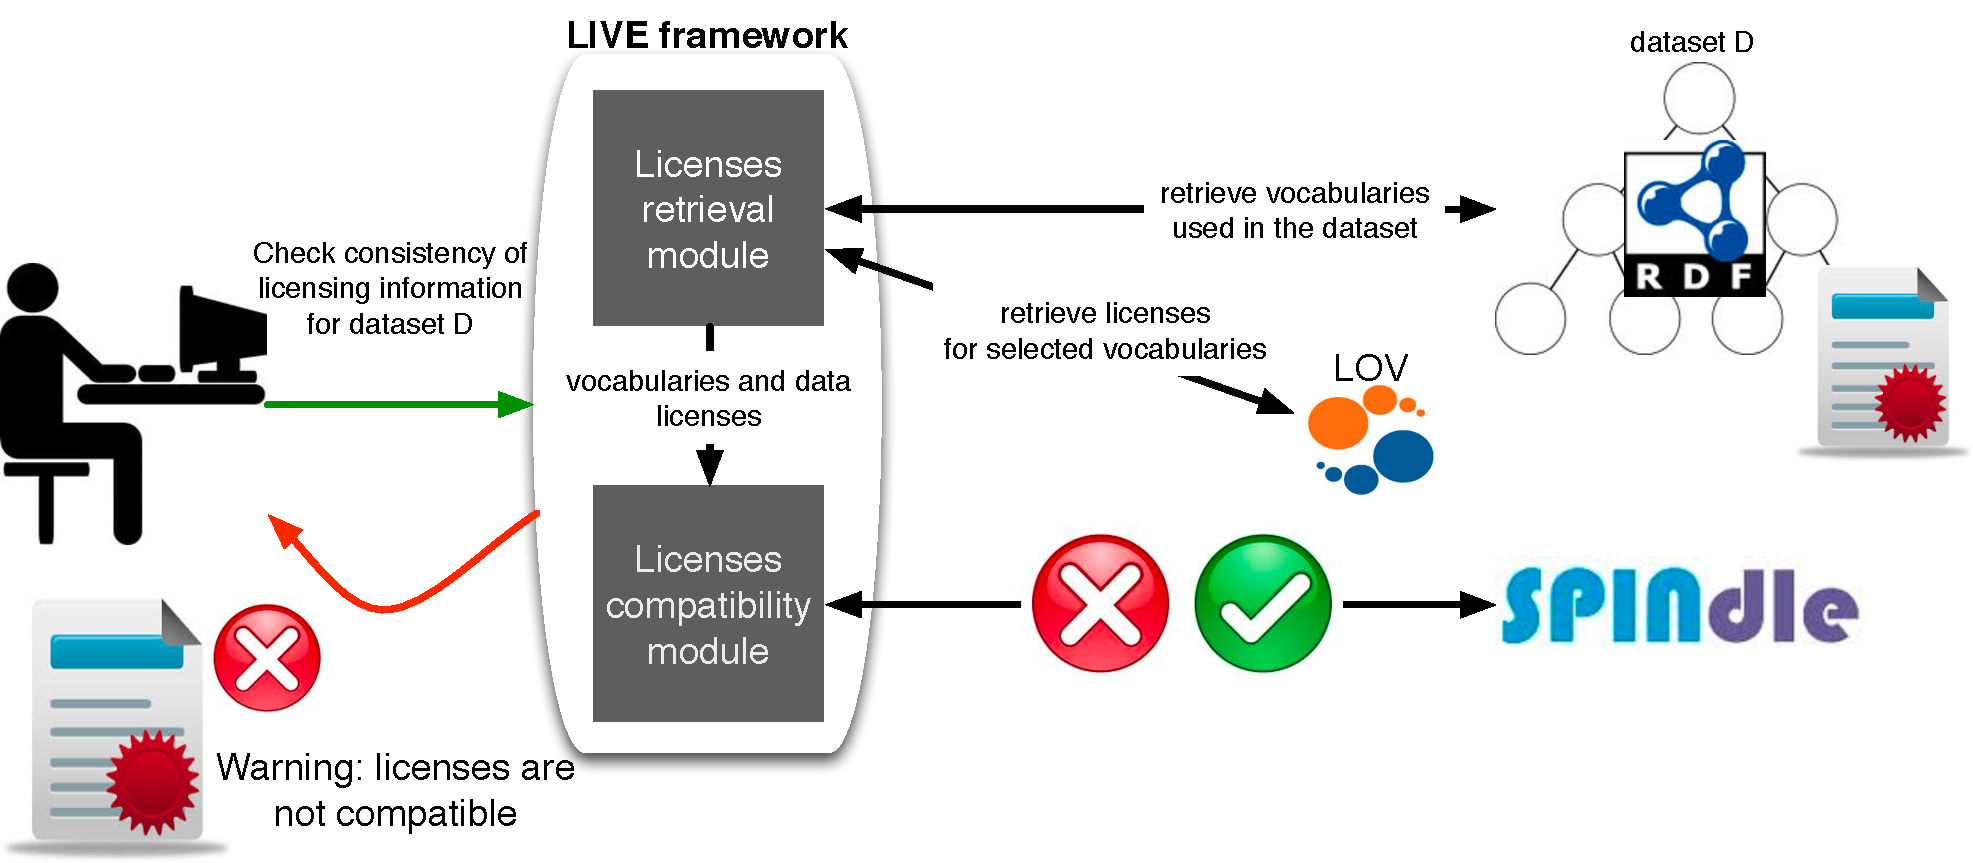
\includegraphics[width=12.0cm]{img/live-framework.pdf}
\caption{LIVE framework architecture.}
\label{fig:framework}
\end{figure}


\subsection{licensing information from vocabularies and datasets.}
Two use-cases are taken into account: a SPARQL endpoint, or a VoID file in Turtle syntax. 
In the first use case, the tool retrieves the named graphs present in the repository, and then the user is asked to select the URI of the graph that needs to be checked. Having that information, a SPARQL query is triggered, looking for entities declared as \texttt{owl:Ontology}, \texttt{voaf:Vocabulary} or object  of the \texttt{void:vocabulary} property. The final step is to look up the LOV catalogue to check whether they declare any license. There are two options for checking the license: \textit{(i)} a \textit{``strict checking'' } where the \texttt{FILTER} clause contains exactly the namespace of the submitted vocabulary, or \textit{(ii)} a \textit{``domain checking''}, where only the domain of the vocabulary is used in the \texttt{FILTER} clause. This latter option is recommended in case only one vocabulary has to be checked for the license. 
%
In the second use case, the module parses a VoID file using a N3 parser for Javascript\footnote{\url{https://github.com/RubenVerborgh/N3.js}}, and then collects the declared vocabularies in the file, querying again LOV\footnote{Since LOV endpoint does not support the JSON format in the results, we have uploaded the data in \url{eventmedia.eurecom.fr/sparql}.} to check their licensing information. 
%
When the URIs of the licenses associated to the vocabularies and the dataset are retrieved, the module retrieves the machine-readable description of the licenses in the dataset of licenses~\cite{CabrioESWC2014}. More specifically, such dataset is composed by 37 licenses, comprising all the licenses adopted to certify data in the Linked Data cloud (as all the Creative Commons licenses\footnote{\url{http://creativecommons.org/licenses/}}), software licenses (as Mozilla Public License\footnote{\url{http://www.mozilla.org/MPL/2.0/}} and Microsoft License\footnote{\url{http://referencesource.microsoft.com/referencesourcelicensing.aspx}}), and additional licenses for other material on the Web (as the UK Open Government license, and the New Free Documentation License\footnote{\url{http://www.gnu.org/copyleft/fdl.html}}). The dataset provides the licenses in RDF using the Turtle syntax, however Creative Commons licenses are also available in XML/RDF format on the CC website\footnote{For instance, Creative Commons Attribution 4.0 license is available at \url{http://creativecommons.org/licenses/by/4.0/rdf}}.
Figure \ref{fig:livetoolUI} shows the user interface for quering a graph and sample results provided by LIVE tool.  

\begin{figure}[ht!b]
\centering{
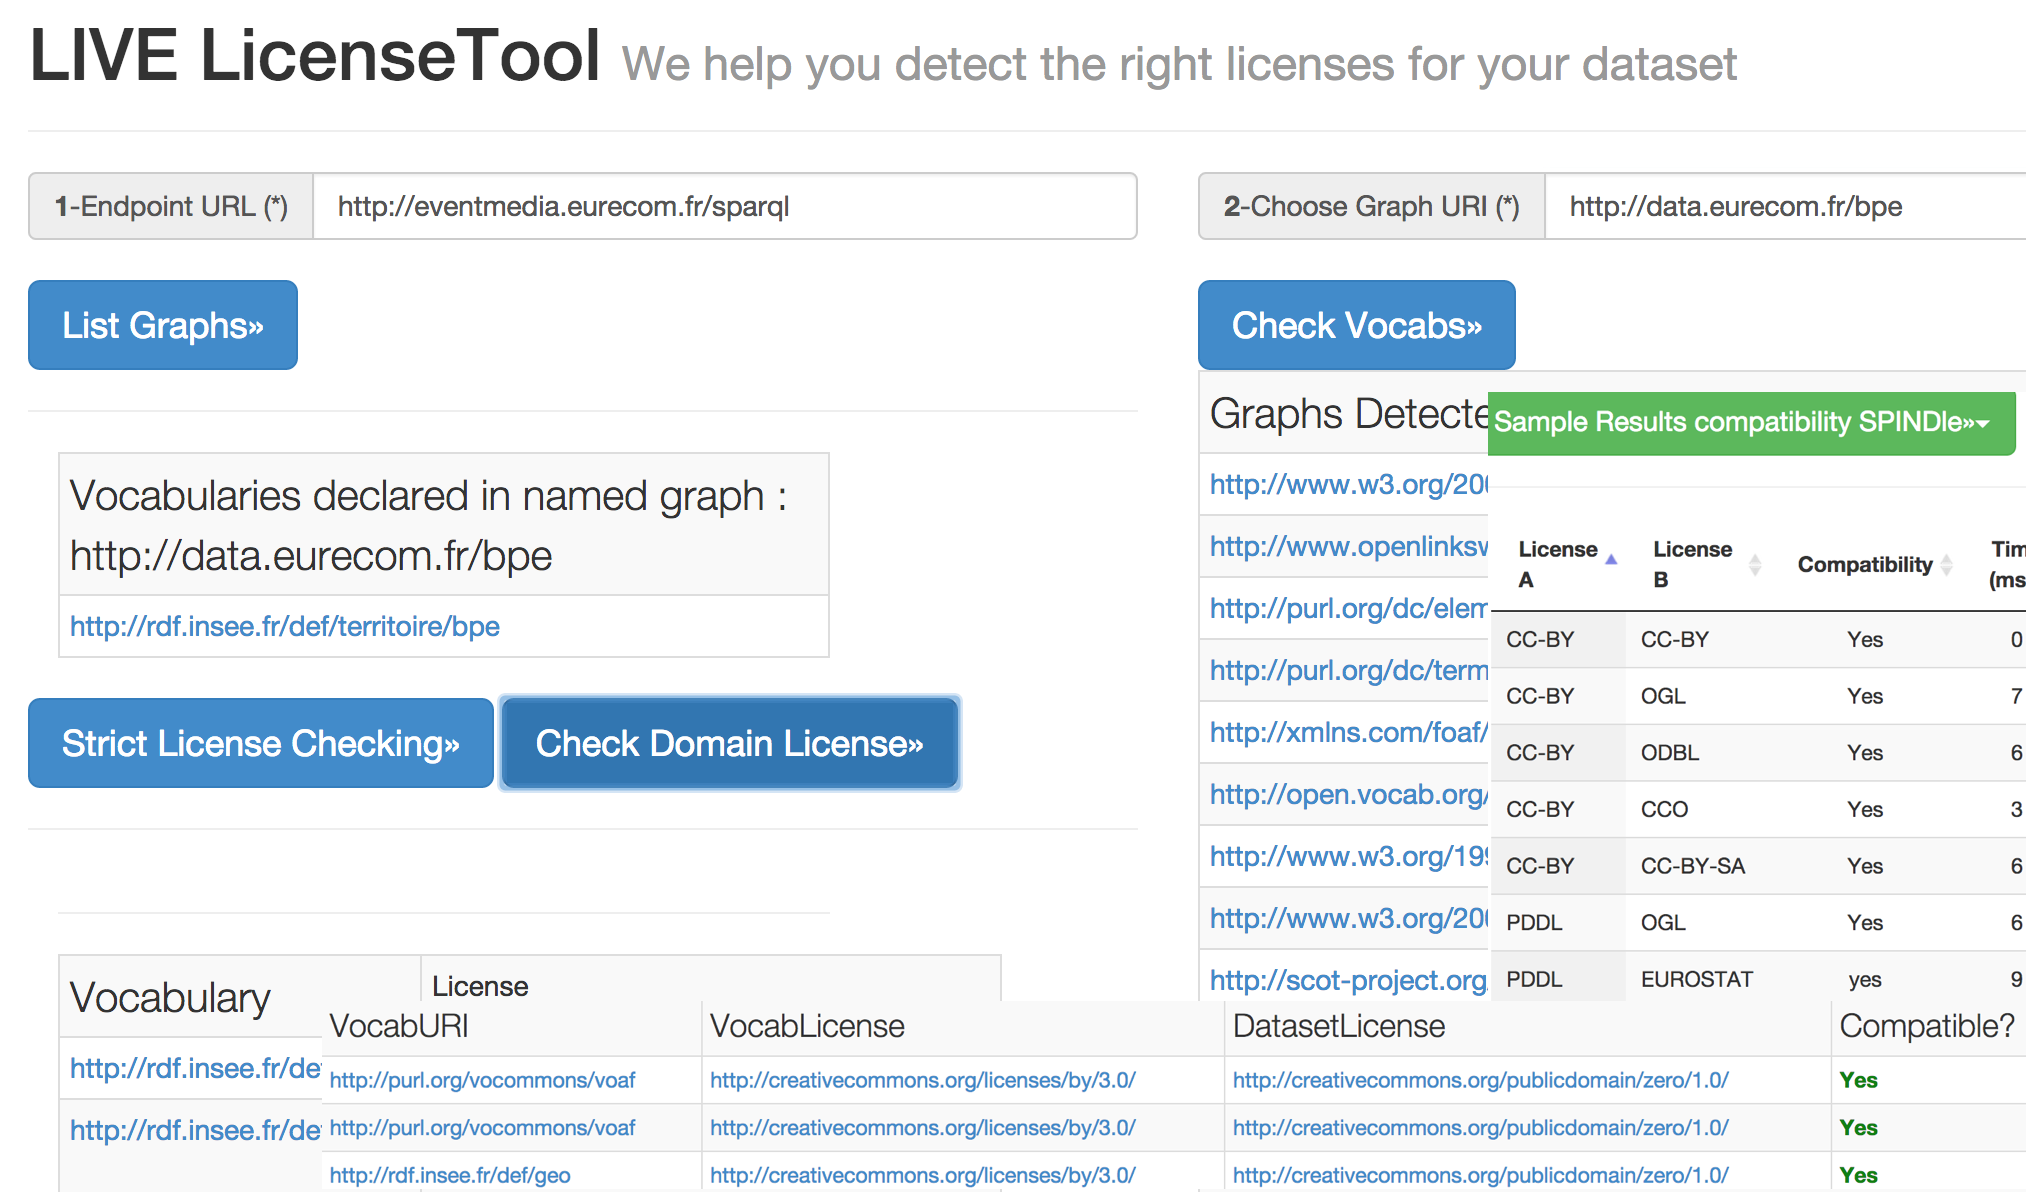
\includegraphics[scale=0.9]{im/LIVETool-UI.png}
\caption{LIVE tool user interface and sample results}
\label{fig:livetoolUI}
}
\end{figure}

\subsection{Licenses compatibility verification.}
The logic proposed in~\cite{DBLP:conf/semweb/GovernatoriRVG13} 
and the licenses compatibility verification process has been implemented using SPINdle~\cite{spindle} 
-- a defeasible logic reasoner capable of inferencing defeasible theories with hundredth of thousand rules.

%
\begin{figure}[ht!]
% \begin{wrapfigure}{r}{.5\textwidth}
\centering{
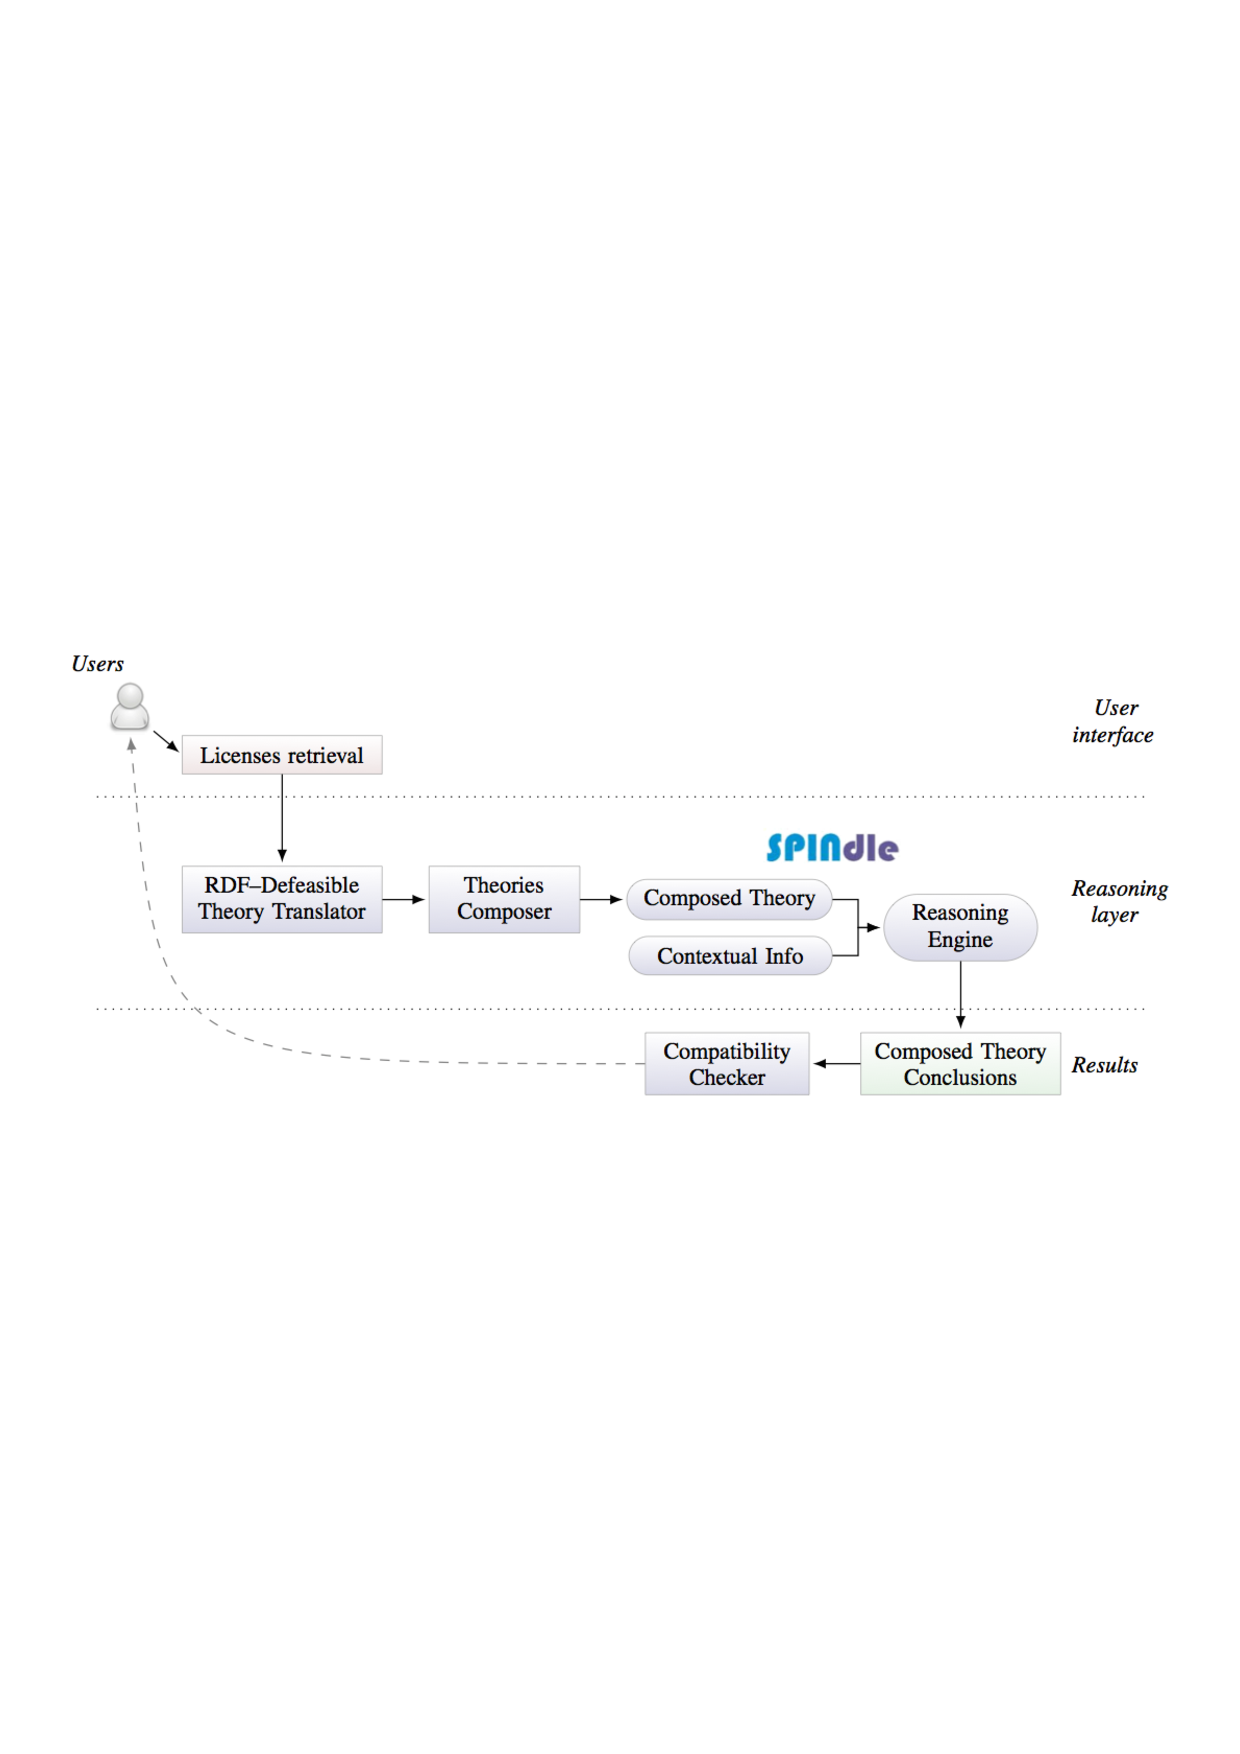
\includegraphics[scale=0.8]{img/composeTheories.pdf}
\caption{Licenses compatibility module.}
\label{figure:theoriesReasoningProcess}
}
\end{figure}
%

As depicted in Figure~\ref{figure:theoriesReasoningProcess},
after receiving queries from users,
the selected licenses (represented using RDF) will be translated into the DFL formalism supported by SPINdle using the \textit{RDF-Defeasible Theory Translator}. 
% If, 
% however,
% more than one license has been selected, % by user,
% then in order to verify the compatibility of different licensing terms, 
% the translated defeasible theories will first be composed into a single defeasible theory~\cite{DBLP:conf/semweb/GovernatoriRVG13} .
That is,
each RDF-triple will be translated into a defeasible rule based on the subsumption relation between the \textit{subject} and \textit{object} of a RDF-triples.
In our case,
we can use the subject and object of the RDF-triples as the antecedent and head of a defeasible rule, respectively.
Besides, 
the translator also supports direct import from the Web and processing of RDF data into SPINdle theories.
%
%the \textit{RDF-Defeasible Theory Translator} will translate the RDF-licenses into the DFL formalism supported by \spindle.

The translated defeasible theories will then be composed into a single defeasible theory based on the logic proposed in~\cite{DBLP:conf/semweb/GovernatoriRVG13},
using the \textit{Theories Composer}.
Afterwards,
the composed theory, 
together with other contextual information (as defined by user),
will be loaded into the SPINdle reasoner to perform a compatibility check before returning the results to the users.

We have evaluated the time performances of the LIVE framework in two steps (Table~\ref{tab:evalTool}).

\begin{table}[ht!]
\centering{
\scriptsize
\begin{tabular}{|l|c|c|c|c|}
\specialrule{1pt}{1pt}{1pt}
 \textbf{Dataset} & \textbf{LicRe-} & \textbf{\#vocabu-} & \textbf{LicCompa-} & \textbf{LIVE(ms)}\\ 
 & \textbf{trieval(ms)} & \textbf{laries} & \textbf{tibility(ms)} & \\ \hline
  rkb-explorer-dblp & 4,499 &  1 & 0 & 4,499\\ \hline
  rkb-explorer-southampton & 14,693 & 1 & 0 & 14,693\\ \hline
  rkb-explorer-eprints & 3,220 & 1 & 0 & 3,220\\ \hline
  rkb-explorer-acm & 3,007 & 1 &  0 & 3,007\\ \hline
  rkb-explorer-wiki & 14,598 & 1 & 0& 14,598\\ \hline
  rkb-explorer-rae2001 & 3,343 & 1 &  0 & 3,343 \\ \hline
  rkb-explorer-citeseer & 2,760 & 1 & 0 & 2,760\\ \hline
  rkb-explorer-newcastle & 3,354 & 1 & 0 & 3,354\\ \hline
  rkb-explorer-kisti & 4,094 & 5 & 6 & 4,100\\ \hline
  270a.info & 13,202 & 48 & 8 & 13,210 \\ \hline
 
\end{tabular}\normalsize
\caption{Evaluation of the LIVE framework.}
\label{tab:evalTool}
}
\end{table}


First, we evaluate the time performances of the licenses compatibility module: it needs about 6ms to compute the compatibility of two licenses. Second, we evaluate time performances (Chrome v. 34) of the whole LIVE framework for the $10$ LOD datasets with the highest number of links towards other LOD datasets, considering both the licenses retrieval module and the licenses compatibility one. The results show that LIVE provides the compatibility evaluation in less than 5 seconds for $7$ of the selected datasets. Time performances of LIVE are mostly affected by the first module while the compatibility module does not produce a significant overhead. For instance, consider Linked Dataspaces\footnote{\url{http://270a.info/}}, a dataset where we retrieve the licensing information in both the dataset and the adopted vocabularies. In this case, LIVE retrieves in $13.20$s $48$ vocabularies, the license for the dataset is CC-BY, and the PDDL license is attached one of the vocabularies\footnote{\url{http://purl.org/linked-data/cube}}. The time for verifying the compatibility is $8$ms, leading to a total of $13.208$s.

\subsection{Future perspectives}
We have introduced the LIVE framework for licenses compatibility. The goal of the framework is to verify the compatibility of the licenses associated to the vocabularies exploited to create a RDF dataset and the license associated to the dataset itself. Several points have to be taken into account as future work. More precisely, in the present paper we consider vocabularies as data but this is not the only possible interpretation. For instance, we may see vocabularies as a kind of compiler, such that, after the creation of the dataset then the external vocabularies are no more used. In this case, what is a suitable way of defining a compatibility verification? We will investigate this issue as well as we will evaluate the usability of the online LIVE tool to subsequently improve the user interface.


\section{Conclusion}
Tell the reader the ``take-away-message'' of this chapter.


